\documentclass[9pt]{IEEEtran}

% basic
\usepackage[english]{babel}
\usepackage{graphicx,epstopdf,fancyhdr,amsmath,amsthm,amssymb,url,array,textcomp,svg,listings,hyperref,xcolor,colortbl,float,gensymb,longtable,supertabular,multicol,placeins}

 % `sumniki' in names
\usepackage[utf8x]{inputenc}

 % search and copy for `sumniki'
\usepackage[T1]{fontenc}
\usepackage{lmodern}
\input{glyphtounicode}
\pdfgentounicode=1
% \usepackage{subfig}
% tidy figures
\graphicspath{{./figures/}}
\DeclareGraphicsExtensions{.pdf,.png,.jpg,.eps}

% correct bad hyphenation here
\hyphenation{op-tical net-works semi-conduc-tor trig-gs}

% ============================================================================================

\title{\vspace{0ex} %
% TITLE IN HERE:
Navigating the government website network using parallel breadth-first crawler
\\ \normalsize{Web Information Extraction and Retrieval 2018/19, Faculty of Computer and Information Science, University of Ljubljana}}
\author{ %
% AUTHOR IN HERE:
Matej Klemen, Andraž Povše, Jaka Stavanja
\vspace{-4.0ex}
}

% ============================================================================================

\begin{document}

\maketitle

\begin{abstract}
BOII
\end{abstract}

\section{Introduction}
[TOLE JE BL ABSTRACT KOKR INTRO IMO]
In this project we have implemented a web crawler in Python programming language. The requirements were, that it only crawls websites ending in ".gov.si", which are Slovenian government websites. The crawler crawls these websites and downloads images and files from them. Visiting new links is performed using Breadth-First search. Website duplicate detection was performed using LSH algorithm. We used Docker to host the database, in which the crawler wrote information into. 
\section{Crawler}
Crawler consists of multiple parts. New link scheduler, making request, scraping the new website for files or images, detecting duplicates and writing data into the database.

PARAMETER THAT OUR CRAWLER TAKES

We used Selenium to make requests, because it also renders the Javascript code on the website. It does, however, not include HTTP status code, which is why we also had to make another request to get that information.


EXPLAIN HOW BREADTH FIRST STRATEGY WORKS
Each worker gets an even share of new links. We then wait for each of the workers to finish and collect the new links they have gathered and place them into the frontier. Afterwards, we repeat the first step and share these new links amongst all workers. With this strategy, we are using Breadth-First approach to visit new websites.


We did not use the database as a frontier storage ----- We stored our frontier in the program itself.

\section{Robots and Sitemaps}
Key element of the crawler is also reading the 'robots.txt' file and sitemap. Based on the robots file, we know whether we can visit a certain link or whether it is not allowed for a crawler to visit that link.
When we read a sitemap, we add all the URLs mentioned in it, into the frontier. 


\section{Database}
The database was build inside a Docker container. We used the same schema, with one minor change, which is adding a column 'lsh\_hash' into the page table. The column stores the value that LSH hash produced for the content of that website. Access to database is made by each worker when he visits a new page. 







\section{Link}


\section{Image and files extracting}
@JAKA --- commnet on the issue with absolute path, very interesting:D

We stored images and files into the file system, since it gives a nicer overview of the gathered information. This was made possible by creating a folder for each new site in which we stored the information. We then stored the location of the file/image into the provided data field in the database.




\section{LSH deduplication}
We implemented LSH algorithm based on CITE CITE CITE. For the words, we use (top 1000 slovenian words???)




\section{Results - 2 seed URLs}

For the sites that are given in the instructions’ seed list and also for the whole crawldb together (for both separately) report general statistics of crawldb (number of sites, number of web pages, number of duplicates, number of binary documents by type, number of images, average number of images per web page, …). Visualize links and include images into the report. If the network is too big, take only a portion of it. Use visualization libraries such as D3js, visjs, sigmajs or gephi.

\section{Results - 9 seed URLs}




\begin{figure}[h] \centering
	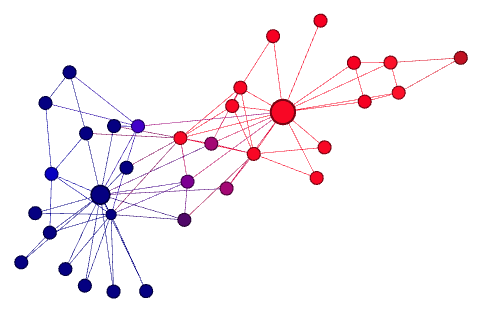
\includegraphics[width=0.4\textwidth]{karate.png}
	\caption{{Example of an image.}}
	\label{fig:karate}
\end{figure}


 
\begin{table}
    \begin{center}
    \caption{Example of a table.}
        \begin{tabular}{ l | r }
        
        Richard Karstark & 0.013661 \\
        Jon Arryn & 0.012869 \\
        Joyeuse Erenford & 0.012869 \\
        Trystane Martell & 0.010761 \\
        Willen Lannister & 0.010684 \\
        Martyn Lannister & 0.010684 \\
        Robb Stark & 0.010304 \\
        Joffrey Baratheon & 0.009875 \\
        Master Caleotte & 0.009495 \\
        Lysa Arryn & 0.009383 \\
        \end{tabular}
    \label{tab:pagerankGOT}
    \end{center}
\end{table}



\bibliographystyle{IEEEtran}
\bibliography{bibliography}


\end{document}